
Similarly to the logic unit, the coincidence unit is a module used to make Boolean operations between signals.\\
%Its inputs are logic pulses and the outputs are logic pulses if pulses appear at all inputs within a time interval (resolving time). In our experiment it is used(as the logic unit) to perform coincidences between signals.\\

The same approach used with the characterization of the logic unit can be applied to the coincidence unit. The setup is shown in Figure \ref{coinc_unit}.\\
\medskip
\medskip
\begin{figure}[!h]
	\centering
	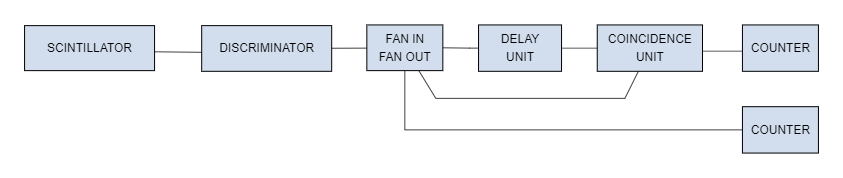
\includegraphics[width=\linewidth]{characterization/coinc_unit}
	\caption{Configuration employed during the coincidence unit characterization.}
	\label{coinc_unit}
\end{figure}
\medskip
\medskip
The fitting function \eqref{eq:fermidirac} that has been employed and errors estimation are completely unvaried with respect to the first characterization of the logic unit. The results are presented below.\\
\medskip
\medskip
\begin{equation}
\begin{array}{l}
f_0 = 0.995 \pm 0.005\\
k = ( 20.936 \pm 9.790 ) \,  \si{ns^{-1}} \\
t_0 = ( 38.100 \pm 0.112 ) \,  \si{ns} .
\end{array}
\end{equation}
\medskip
\medskip
and the covariance matrix is
\begin{equation}
\textrm{C}=\left(
\begin{array}{ccc}
     2.24 \cdot 10^{-5}  &  -1.39\cdot 10^{-2} &  -1.59 \cdot 10^{-4} \\
    -1.39 \cdot 10^{-2} &      95.84  &      0.98\\
    -1.59\cdot 10^{-4}  &       0.98   &    1.26\cdot 10^{-2} 
\end{array}
\right)
\end{equation}
The accordance between data and the model is excellent since $P_8\left(\chi^2\geq\chi_{obs}^2\right)=99.96\,\%$.
It can be observed that  the counts fall sharply around a certain value of delay and almost no counts are registered for delays greater than this one.  
The value of this delay is about $\SI{38.1}{ns}$ and the obtained time width for the coincidence unit is: 
\begin{equation}
\delta_T = ( 0.191\pm 0.089 ) \, \si{ns}.
\end{equation}
The relative uncertainty obtained on $\delta_T$ is quite big $\left( \delta_{\delta_T} / \delta_T \sim 46.6 \%\right)$ since the decrease of the function is steep and a few data have been sampled in this region.\\

\begin{figure}[!h]
	\centering
	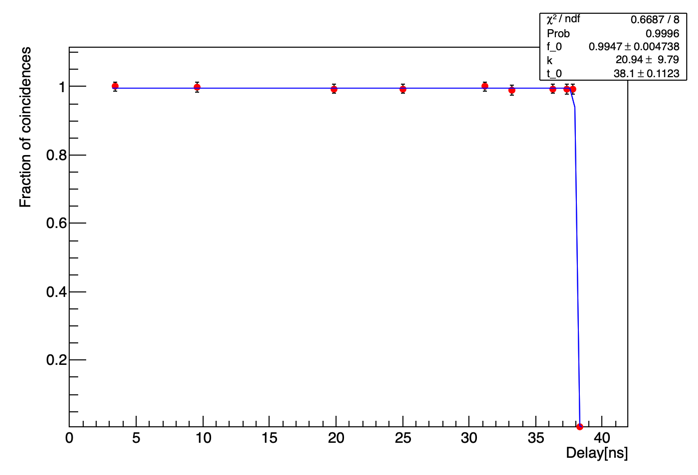
\includegraphics[width=.75\linewidth]{characterization/coinc_plot}
	\caption{Coincidence unit characterization.}
	\label{coinc_plot}
\end{figure}

